\chapter{Development environment}\label{chap:editor}
The goal is to build an online \acrlong{ide} IDE, similar to
Codeanywhere\footnote{\url{https://codeanywhere.com/}} or
Cloud9\footnote{\url{https://c9.io/}}, works offline as well.

\section{Overview}
A folder is considered a project, similarly to modern code editors, such as
Brackets or Visual Studio Code.

The current version of the development environment is intended to be used
offline, on user's machine. Nevertheless it is designed so that it could be
easily transformed into an online system.

I decided to implement the system with minimal dependencies, so it can be easily
installed and so I can achieve a greater level of integration by having more
control over every part.

The only required dependency for the basic functionality of the prototype to
work (which is the editor) is a web browser and the CodeMirror library. An
additional dependency is the Node.js environment.

The language's development environment is implemented as a web application. It
consists of three parts:
\begin{itemize}
    \item The server part, implemented in JavaScript on top of Node.js. This
      part's functions is mainly to enable access to user's file system, so any
      local folder can be opened as a project -- modern web browsers restrict
      access to the local file system, because of security reasons. The server
      part also handles persisting changes to files and configuration.
    \item The project manager part, which communicates directly with the server
      part. The connection is maintained over a
      WebSocket\footnote{\url{https://developer.mozilla.org/pl/docs/WebSockets}}. This
      part provides access to user's file system via a custom folder selection
      interface. Basic configuration of server communication, such as changing
      the address and ports is also possible. Once a project is selected, the
      user may open it in the editor part.
    \item The editor part, which is the main component and can function as a
      stand-alone application. It can communicate with the server indirectly,
      through the \texttt{localStorage}
      mechanism\footnote{\url{https://developer.mozilla.org/en-US/docs/Web/API/Window/localStorage}}.
\end{itemize}

The project manager and the editor, which can be considered the front-end parts
of the system are designed to be a
\acrlong{spa}\footnote{\url{https://en.wikipedia.org/wiki/Single-page_application}}. The
project manager exchanges JSON messages with the server through a
WebSocket. This is used for updating the view with dynamic data. In order to
facilitate the manipulation of the HTML structure of the page, which is the main
application's view, I implemented a very simple web application framework, which
binds the data from the server with the data on the client and the
\acrlong{dom}\footnote{\url{http://eloquentjavascript.net/13_dom.html}}.

\begin{figure}[h!]
\centering 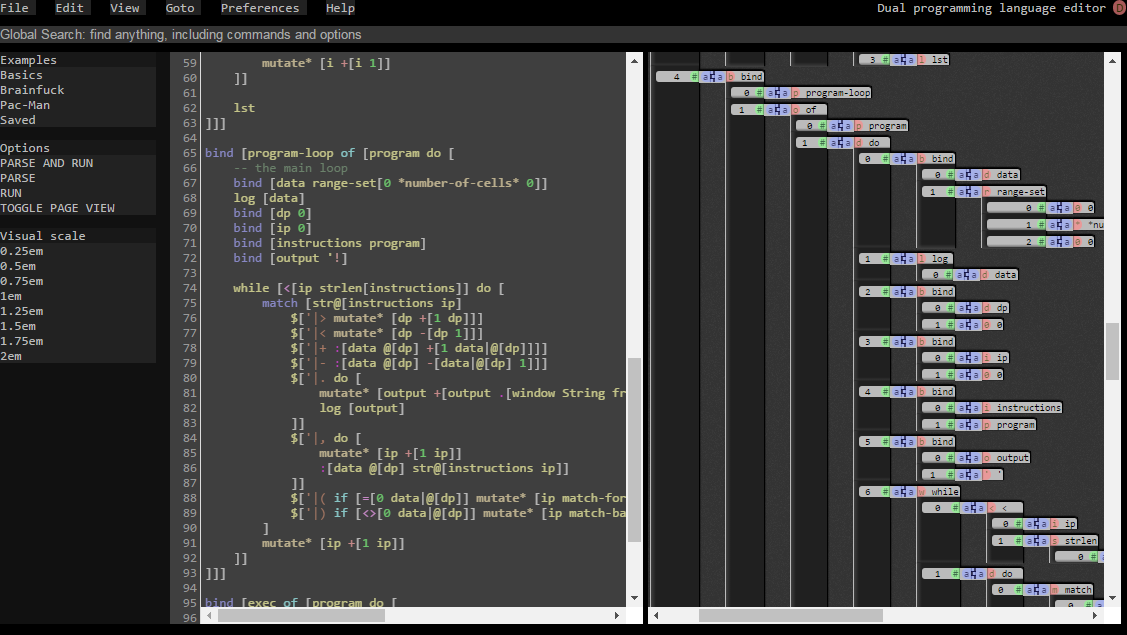
\includegraphics[width=0.9\textwidth]{editor}
\caption{The editor}
\label{fig:editor}
\end{figure}

Figure \ref{fig:editor} shows an overview of the editor prototype's window. The
basic layout is modeled after the aforementioned code editors. At the top of the
window is the menu bar, below a global search input (not implemented in the
prototype). The left panel contains basic controls for selecting examples,
invoking the parser and interpreter, toggling application view and adjusting the
scale of the visual representation.

The following options are implemented in the prototype:
\begin{itemize}
    \item Available from the menu bar:
    \begin{itemize}
        \item File->Save, which saves the current content of the text editor to
          a file named \texttt{save.dual} in editor's root directory. This only
          works if the server-side part of the environment is running. Otherwise
          the source will be saved only to browser's internal storage.
        \item In the Edit menu: Undo, Redo, Cut, Copy, Paste and Select All
          options are supported. Note that by default web browsers restrict the
          access to the user's clipboard, so for Copy and Paste the standard key
          shortcuts should be used (Ctrl-C, Ctrl-V). All other conventional
          keyboard shortcuts are also supported, thanks to the CodeMirror
          library.
    \end{itemize}
    \item Available from the left panel:
    \begin{itemize}
        \item The options in the Examples submenu cause a corresponding source
          file to be loaded into the editor. This is for demonstration for the
          purposes of this thesis.
        \item The Options submenu allows the user to invoke the parser and the
          interpreter separately or in combination as well as toggling between
          the ``page'' (also known as ``application'') and visual editor
          views. The application view contains an embedded web page (iframe),
          which can be manipulated by a Dual application. This is used to
          display the game view in the Pac-Man clone example.
        \item The Visual scale submenu changes the size of the blocks in the
          visual editor. This demonstrates how manipulating one CSS property
          influences the rendering of the visual representation.
    \end{itemize}
\end{itemize}

Some options have descriptive captions available that appear when the mouse
cursor hovers over them.

\section{Text editor}
The text editor is built on top of the CodeMirror
framework\footnote{\url{https://codemirror.net/}}. It was integrated with the
editor in the following way:
\begin{itemize}
    \item A custom syntax highlighting mode for Dual was defined.  % crucial:
    \item If a position of the text cursor in or the contents of the source
      change, a fragment of text corresponding to the appropriate \acrshort{est}
      node is highlighted. Also the corresponding subtree in the visual editor
      is highlighted. This works also in the other direction -- when a node in
      the visual editor is selected, it is highlighted along with the
      corresponding text fragment. This demonstrates the core functionality of
      the system: it is ``aware'' at all times of currently focused meaningful
      part of the code, corresponding to an \acrshort{est} node. This is
      reflected in every representation that is associated with the EST.

\end{itemize}
Because every node in the EST is linked in both directions with a corresponding
abstract element in a representation, any change to the element can be reflected
in the node and, through the EST, in all other associated representations. This
makes the system accurate and fast, as every change happens in an isolated
context, which doesn't have to be reestablished every time a modification is
made.

We can distinguish three representations used by the system:
\begin{enumerate}
    \item The EST, which is the master representation of the program.
    \item The fragments of text corresponding to EST nodes in the text
      representation are tracked by CodeMirror's TextMarker objects. These
      facilitate tracking and propagating any changes to and from this
      representation, as well as highlighting.
    \item The visual representation, which is implemented in terms of pure HTML
      tables fully styled with CSS. This allows for easy and complete
      customization of the representation.
\end{enumerate}

\begin{figure}[h!]
\centering 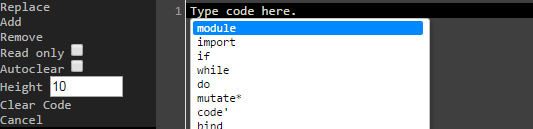
\includegraphics[width=0.9\textwidth]{editor-menu}
\caption{Visual editor's context menu}
\label{fig:editor-menu}
\end{figure}

In case of the visual representation this is implemented in a rather
straightforward way: every EST node has a corresponding set of \acrshort{dom}
nodes. Thanks to this, we can track any actions performed on the DOM through the
standard browser-implemented interface. This is solved in the prototype by
attaching \texttt{click} event handlers to relevant nodes. Such an event
triggers the following:
\begin{itemize}
    \item A corresponding EST node is ``focused'' by the system.
    \item A context menu appears similar to that depicted in
      \ref{fig:editor-menu}. This menu has basic options for editing the visual
      nodes: Replace, Add and Remove. These perform their corresponding action
      on the currently focused node and propagate it to all representations. The
      Remove option simply removes the selected node and its subtree from the
      DOM, the EST, as well as the associated text fragment. Add and Replace
      make use of the small text-editor area next to the context menu. It
      contains a list of possible names of nodes to be inserted in case the user
      wants to a node. Selecting any of the names causes a template for the new
      node (in the form of an editable code snippet) to be inserted into the
      text-editor area. Such a template can be quickly adjusted by the user
      before inserting. The user may also type in raw code into the text box,
      without selecting any templates. After entering the code and selecting the
      appropriate option, the text is parsed, transformed into TextMarker, EST
      and DOM representations. Then all the versions of the fragment are
      inserted in appropriate places.
\end{itemize}

The list of possible nodes displayed along with the context menu is implemented
in terms of a simple autocomplete functionality on top of CodeMirror. Every item
in the autocomplete list is associated with a fragment of code, which is
basically a signature of the corresponding function. User-defined functions
could be easily automatically added to this list by extracting their signatures
from definitions. Autocompletion should also be made context-sensitive,
similarly to modern code editors.

The templates could also be selected by the user from a visual library of puzzle
pieces, like the one in Scratch (Fig. \ref{fig:scratch}).
\begin{figure}[h!]
\centering 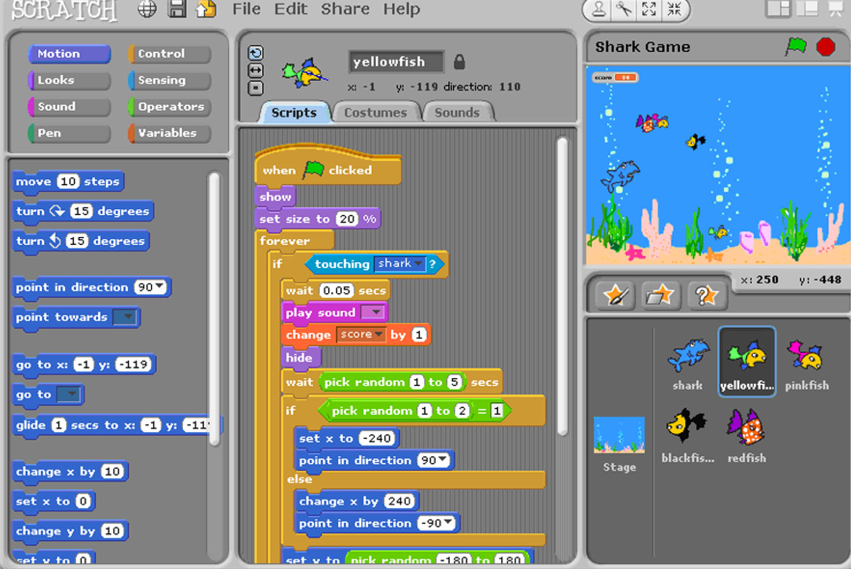
\includegraphics[width=0.9\textwidth]{scratch}
\caption{ MIT Scratch programming language editor\protect\footnote{ Screenshot
    from \url{
      http://mypad.northampton.ac.uk/12406702/files/2013/05/Screen-Shot-2013-05-02-at-23.19.19-1s0qp26.png
} } }
\label{fig:scratch}
\end{figure}


\section{Visual editor}
\subsection{The visual representation}
The design of Dual's visual representation draws from many visual programming
languages. Analyzing these, we can observe several distinct approaches of which two particular designs are the most widespread and successful. These can be
described as ``line-connected block-based'' and ``snap-together block-based''
visual languages. The former family is exemplified by the Blueprints Visual
Scripting system of Unreal Engine 4\cite{blueprint} and the latter by MIT Scratch\cite{scratch, scratch_wikipedia}.


Basic design principles: make it no harder to use than the textual
representation ideally it should add useful capabilities, without taking away
these provided by text editors

Existing visual languages are mostly criticized, because they fail to meet these
basic criteria.

\subsubsection{Flexibility}
The fact that the visual representation is composed purely out of HTML and CSS
Fully customisable with CSS

\subsubsection{Design}
\begin{figure}[h!]
\centering 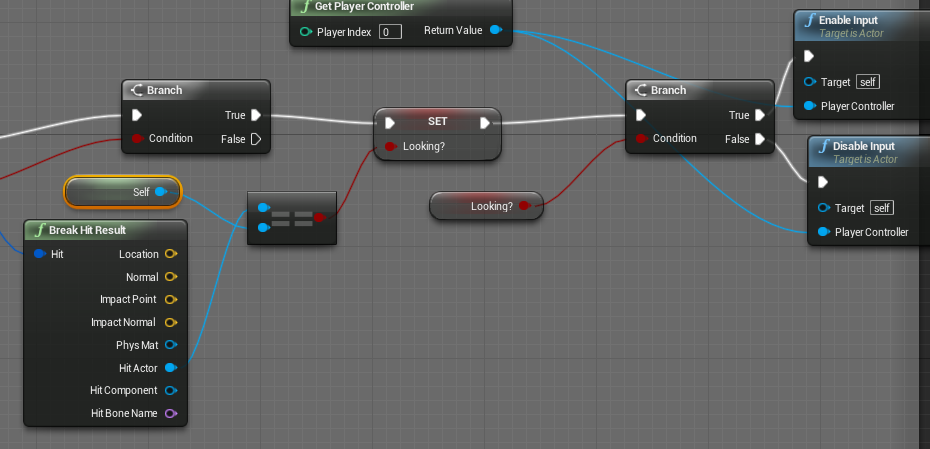
\includegraphics[width=0.9\textwidth]{blueprint_more}
\caption{}
\label{fig:blueprint_more}
\end{figure}

Many iterations:

\begin{figure}[h!]
\centering 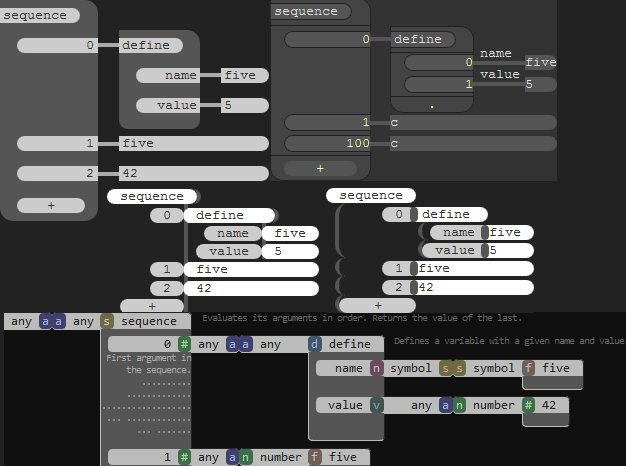
\includegraphics[width=0.9\textwidth]{designs_01234}
\caption{}
\label{fig:designs_01234}
\end{figure}

The visual form allows us to provide much more information about different
elements of the program.  Spatially relate this information with these elements
through blocks and connections.  Relate expressions with other expressions
through connections, which can also carry additional information.

We can distinguish the following visual elements:
\begin{itemize}
	\item Blocks, which represent expressions or individual nodes of the
          EST. Those in turn consist of:
	\begin{itemize}
		\item A header, which contains an icon and the name of the
                  expression's operator. Next to the header a documentation
                  comment might be displayed.
		\item Slots, which are the numbers or names of the arguments
                  followed by an icon; below these documentation comments could
                  be displayed.
		\item Possibly additional buttons, which could be used to add
                  more slots to variadic expressions.
	\end{itemize}
	\item Connections between slots and blocks, which could also contain
          some useful annotations. The proposed design places type annotations
          there. These consist of the name of the type followed by an icon that
          represents this type. Connections actually have two parts: one
          extending from a slot, which in this case would contain the argument's
          type annotation, and one extending from a block header, which would
          contain expression return value's type annotation.
\end{itemize}

Icons are a way to minimize the use of text to represent different entities

The text representation is very compact, which often is an advantage. This
advantage can be maintained by the visual representation by making all the
additional information optional. The user should have easy way of configuring
whether or not and what informations should be displayed. By folding some
textual elements into icons the visual representation could actually be made
more compact than the text form.

\subsubsection{Structure}
The programmer could have the ability to alter the structure of the
representation, but he should not be required to constantly shape it. A
connected-block representations, such as the one in Unreal Engine 4 has no
mechanism that automatically structures the visual code similar to
autoindentation and other useful autostructuring features that evolved in code
editors over time and experience with using text-based programming
languages. This can be considered a regression on the visual editors' part.

The early designs show the following features that are not implemented in the
final prototype:
\begin{itemize}
	\item Names of the arguments are displayed instead of numbers if
          sensible.
	\item Names of types of variables
\end{itemize}

The colored squares with letters inside are actually placeholders for icons.  I
imagine a design, where the user is able to click on those icons and fold the
blocks into a more compact form, hiding the names and excessive text. This could
be done on the level of individual blocks, whole subtrees or the entire program
-- similar to code folding in text editors. This allows to have a big picture
and general relationships between nodes always visible and at the same time
gives an ability to focus on the details of the part at hand.

The text below the slots could be documentation comments associated with the
given argument. Their visibility could be toggleable through clicking on them,
on an individual or global basis, similarly to icons.

We can observe that there's a need to manipulate or set visual properties of
individual objects, clusters of objects/subtrees as well as the entire program
tree.


\begin{figure}[h!]
\centering 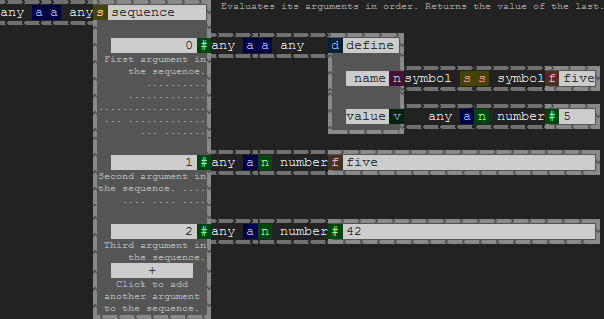
\includegraphics[width=0.9\textwidth]{design_3}
\caption{This design has the interesting property of visually illustrating the
  program flow with arrows.}
\label{fig:design_3}
\end{figure}


\begin{figure}[h!]
\centering 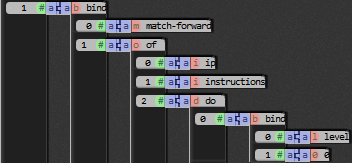
\includegraphics[width=0.9\textwidth]{design_4}
\caption{}
\label{fig:design_4}
\end{figure}

\section{Performance}
It could be optimized similarly to CodeMirror or other web-based text editors or
applications. That is, only a visible portion (plus a margin, which allows for
fast scrolling) of the code is rendered as DOM nodes at any time. The scrollbar
is virtual and controlled by the editor rather than the browser.

Text editors like CodeMirror use similar amount of DOM nodes [[]], but thanks to
these optimizations are able to handle
megabyte-sized\footnote{\url{http://codemirror.net/doc/internals.html\#approach}}
text files and are used in many real-world
applications\footnote{\url{http://codemirror.net/doc/realworld.html}}, which
includes being a built-in editor in developer tools in major web browsers.

Another source of inefficiency is that parsing is done twice -- once by Dual's
parser and once by CodeMirror's system, which are incompatibile.  A solution to
that would be to implement a custom text editor or extend/modify CodeMirror to
work with Dual's parser.


\begin{figure}[h!]
\centering 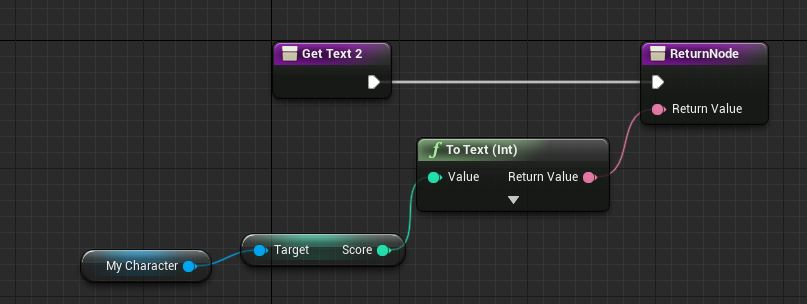
\includegraphics[width=0.9\textwidth]{blueprint}
\caption{Blueprints Visual Scripting\protect\footnote{Screenshot from
    \url{https://docs.unrealengine.com/latest/images/Engine/Blueprints/HowTo/BPHT_6/GetScore.jpg}}}
\label{fig:blueprint}
\end{figure}

\section{Comparison}
% also show that Scratch is inferior, e.g. having no first-class functions
% mention that there are derivatives that try to fix that